\documentclass[12pt,a4paper]{article}

% ============================================================
% PACKAGES
% ============================================================
\usepackage[
    a4paper,
    top=1.55cm,
    bottom=1.35cm,
    left=1.75cm,
    right=1.75cm
]{geometry}

\usepackage[T1]{fontenc}
\usepackage{newtxtext}
\usepackage{graphicx}
\usepackage{xcolor}
\usepackage{array}
\usepackage{tabularx}
\usepackage{fancyhdr}
\usepackage{tikz}
\usepackage{eso-pic}
\usepackage{ragged2e}

% ============================================================
% COLORS
% ============================================================
\definecolor{GEUBlue}{RGB}{43,91,145}
\definecolor{GEUBannerBlue}{RGB}{0,102,148}
\definecolor{GEUYellow}{RGB}{255,201,38}
\definecolor{InstructionGrey}{RGB}{125,125,125}

% ============================================================
% GENERAL SETTINGS
% ============================================================
\setlength{\parindent}{0pt}
\setlength{\parskip}{0pt}
\renewcommand{\arraystretch}{1}

% ============================================================
% HEADER / FOOTER
% ============================================================
\pagestyle{fancy}
\fancyhf{}

\fancyhead[L]{%
    \fontsize{10.5}{12}\selectfont
    B.TECH (CSE) - DSCPP-III-2026-T078
}

\fancyhead[R]{%
    \fontsize{10.5}{12}\selectfont
    PHASE-II PROJECT PROGRESS
}

\fancyfoot[R]{%
    \fontsize{10}{12}\selectfont
    Page \thepage
}

\renewcommand{\headrulewidth}{0pt}
\renewcommand{\footrulewidth}{0pt}

\setlength{\headheight}{20pt}
\setlength{\headsep}{0.65cm}
\setlength{\footskip}{0.65cm}

% ============================================================
% BOTTOM YELLOW LINE
% ============================================================
\AddToShipoutPictureBG{%
\begin{tikzpicture}[remember picture,overlay]
    \fill[GEUYellow]
    (current page.south west)
    rectangle
    ([yshift=0.14cm]current page.south east);
\end{tikzpicture}
}

% ============================================================
% CUSTOM COMMANDS
% ============================================================
\newcommand{\sectiontitle}[1]{%
    {\color{GEUBlue}
    \fontsize{18}{22}\selectfont #1}
}

\newcommand{\instruction}[1]{%
    {\color{InstructionGrey}
    \fontsize{10.5}{13}\selectfont #1}
}

\newcommand{\answerbox}[2]{%
    \begin{tabularx}{\textwidth}{
        |>{\raggedright\arraybackslash}X|}
        \hline
        \parbox[t][#1][t]{\dimexpr\linewidth-12pt\relax}{
            \vspace{5pt}
            \fontsize{11}{13}\selectfont #2
        }\\
        \hline
    \end{tabularx}
}

% ============================================================
% DOCUMENT
% ============================================================
\begin{document}

% ============================================================
% PAGE 1
% ============================================================

\vspace*{0.10cm}

% Upload Graphic Era logo as graphicera_logo.png
\includegraphics[width=8.0cm]{geulogo.png}

\vspace{0.70cm}

\noindent
\colorbox{GEUBannerBlue}{%
\parbox{\dimexpr\textwidth-2\fboxsep\relax}{
    \vspace{0.17cm}
    {\color{GEUYellow}
    \fontsize{16.5}{20}\selectfont
    \bfseries
    PROJECT AND TEAM INFORMATION}
    \vspace{0.17cm}
}}

\vspace{0.80cm}

% PROJECT TITLE
\sectiontitle{Project Title}

\vspace{0.05cm}

% \instruction{(Try to choose a catchy title. Max 20 words).}

\vspace{0.40cm}

\answerbox{1.00cm}{TapNGo - A Bus Fare Verification And Payment System}

\vspace{0.80cm}

% STUDENT INFORMATION
% \sectiontitle{Student/Team Information}

% \vspace{0.40cm}

% \begin{tabularx}{\textwidth}{
% |>{\raggedright\arraybackslash}p{0.66\textwidth}
% |>{\raggedright\arraybackslash}X|
% }
% \hline

% \parbox[t][1.15cm][t]{\linewidth}{
% \vspace{4pt}
% \fontsize{10.5}{13}\selectfont
% Team Name:\\[2pt]
% Team \# (Mentor needs to assign)
% }
% &
% \\
% \hline

% \parbox[t][3.65cm][t]{\linewidth}{
% \vspace{5pt}
% \fontsize{10.5}{13}\selectfont
% Team member 1 (Team Lead)\\[3pt]
% {\color{InstructionGrey}
% (Last Name, name: student ID: email, picture):}
% }
% &
% \\
% \hline

% \parbox[t][3.65cm][t]{\linewidth}{
% \vspace{5pt}
% \fontsize{10.5}{13}\selectfont
% Team member 2\\[3pt]
% {\color{InstructionGrey}
% (Last Name, name: student ID: email, picture):}
% }
% &
% \\
% \hline

% \end{tabularx}

% \newpage
\noindent
\begin{tabularx}{\textwidth}{|>{\RaggedRight\arraybackslash}p{0.69\textwidth}|>{\RaggedRight\arraybackslash}X|}
\hline
\begin{minipage}[t]{\linewidth}
\vspace{1.5mm}
\textit{Team Name:}\\[-1mm]
\textit{Team \#}
\vspace{1.5mm}
\end{minipage}
&
\begin{minipage}[t]{\linewidth}
\vspace{1.5mm}
\textit{Avengers}
\vspace{1.5mm}
\end{minipage}
\\
\hline
\begin{minipage}[t][3.25cm][t]{\linewidth}
\vspace{1.5mm}
\textbf{Team member 1 (Team Lead)}\\[-1mm]
\textit{(Last Name, name: student ID: email, picture):}
\vspace{2.0cm}
\end{minipage}
&
\begin{minipage}[t][3.25cm][t]{\linewidth}
\vspace{1.5mm}
\textup{Jain, Karnika -- 2510010541}\\
\textup{karnikajain90@gmail.com}

\vspace{2mm}
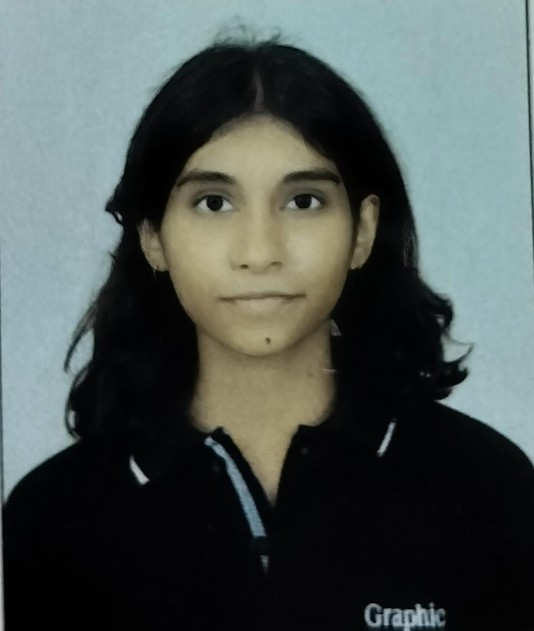
\includegraphics[width=3.0cm,height=1.5cm,keepaspectratio]{member1.png}
\end{minipage}
\\
\hline
\begin{minipage}[t][3.25cm][t]{\linewidth}
\vspace{1.5mm}
\textbf{Team member 2}\\[-1mm]
\textit{(Last Name, name: student ID: email, picture):}
\vspace{2.0cm}
\end{minipage}
&
\begin{minipage}[t][3.25cm][t]{\linewidth}
\vspace{1.5mm}
\textup{Bahuguna, Anirudh -- 2510013536}\\
\textup{anirudhbahuguna14@gmail.com}

\vspace{2mm}
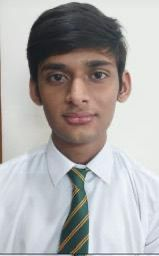
\includegraphics[width=3.0cm,height=1.5cm,keepaspectratio]{member2.png}
\end{minipage}
\\
\hline
\begin{minipage}[t][3.25cm][t]{\linewidth}
\vspace{1.5mm}
\textbf{Team member 3}\\[-1mm]
\textit{(Last Name, name: student ID: email, picture):}
\vspace{2.0cm}
\end{minipage}
&
\begin{minipage}[t][3.25cm][t]{\linewidth}
\vspace{1.5mm}
\textup{Budakoti, Aaditya -- 2510290931}\\
\textup{aadityabudakoti@gmail.com}

\vspace{2mm}
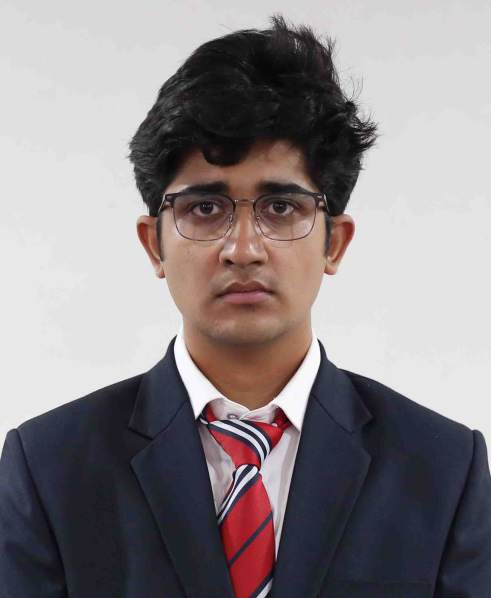
\includegraphics[width=3.0cm,height=1.5cm,keepaspectratio]{member3.png}
\end{minipage}
\\
\hline
\begin{minipage}[t][3.25cm][t]{\linewidth}
\vspace{1.5mm}
\textbf{Team member 4}\\[-1mm]
\textit{(Last Name, name: student ID: email, picture):}
\vspace{2.0cm}
\end{minipage}
&
\begin{minipage}[t][3.25cm][t]{\linewidth}
\vspace{1.5mm}
\textup{Pant, Aparajita -- 2510011139}\\
\textup{aparajitapant246@gmail.com}
\vspace{2mm}
 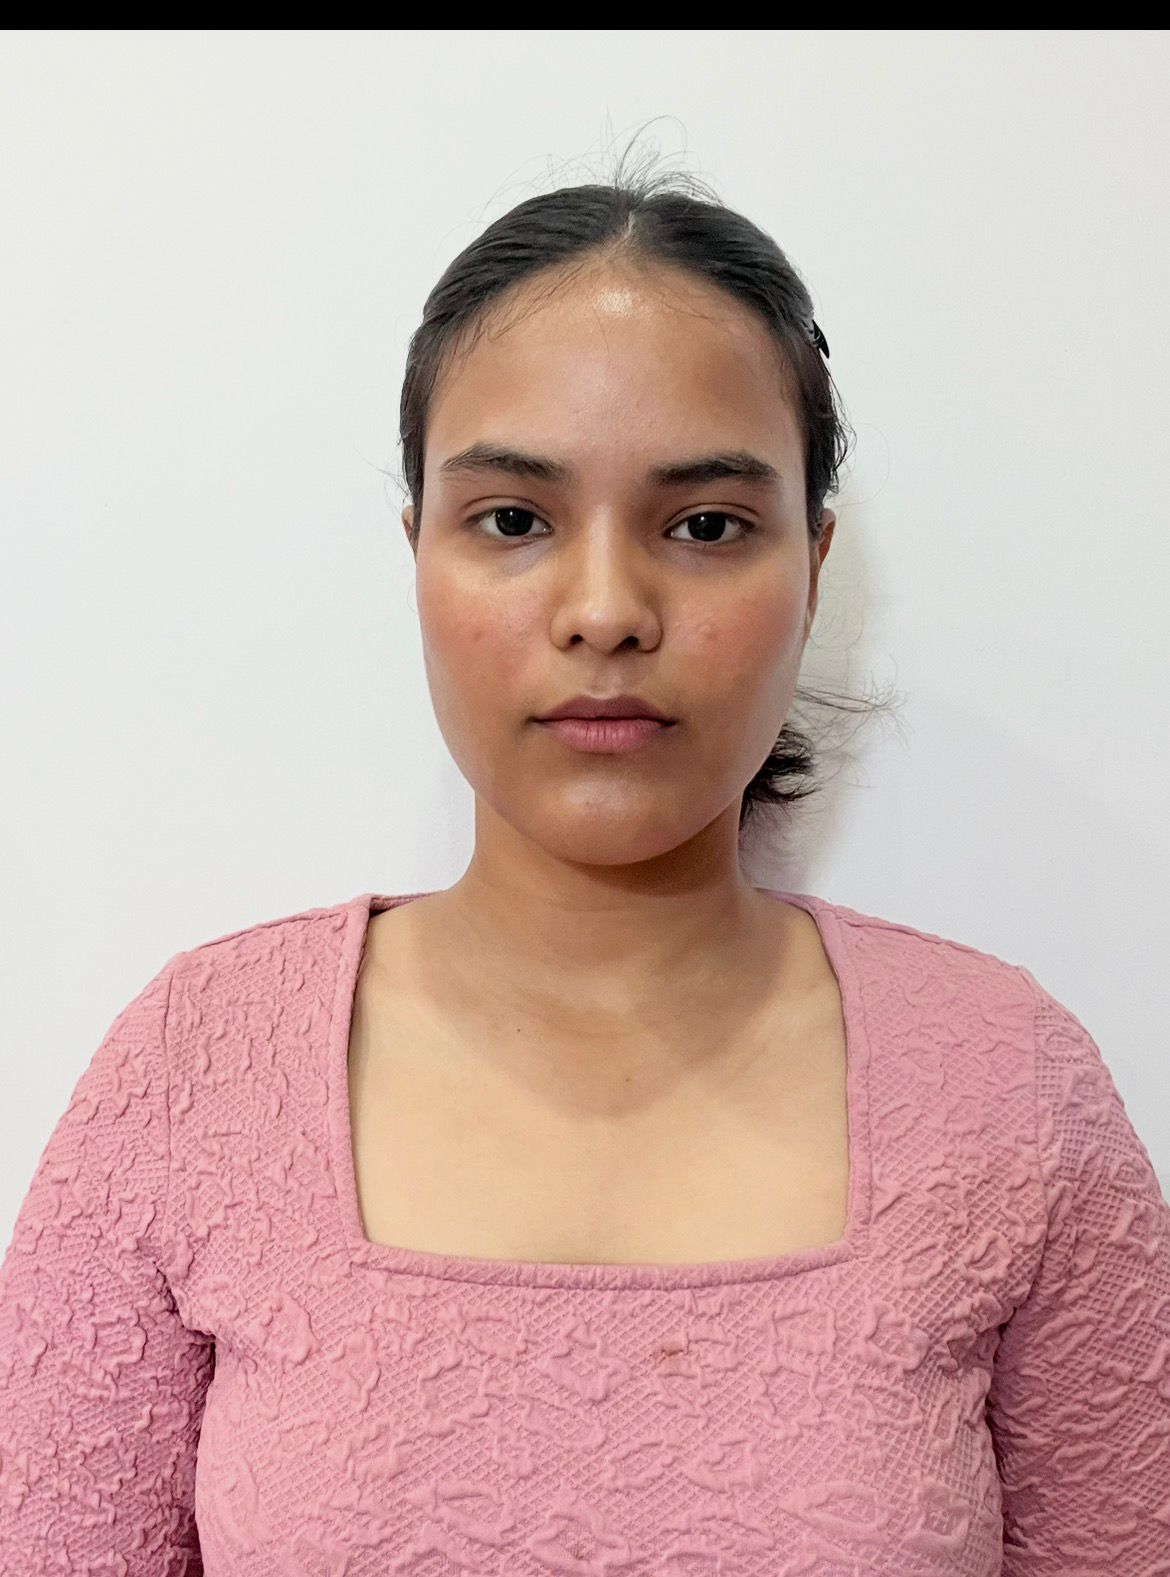
\includegraphics[width=3.0cm,height=1.5cm,keepaspectratio]{member4.png}
\end{minipage}
\\
\hline
\end{tabularx}

\newpage
% ============================================================
% PAGE 2
% ============================================================

\vspace*{0.15cm}

\noindent
\colorbox{GEUBannerBlue}{%
\parbox{\dimexpr\textwidth-2\fboxsep\relax}{
    \vspace{0.18cm}
    {\color{GEUYellow}
    \fontsize{17}{21}\selectfont
    \bfseries
    PHASE-II PROJECT PROGRESS DESCRIPTION (35 pts)}
    \vspace{0.18cm}
}}

\vspace{0.70cm}

% PROJECT ABSTRACT
\sectiontitle{Project Abstract (2 pts)}

\vspace{0.05cm}

% \instruction{(Brief restatement of your project's main goal. Max 300 words).}

\vspace{0.12cm}

\answerbox{6cm}{Our project TapNGo is an automated bus fare verification and seat monitoring system which is designed to help reduce boarding delays due to manual fare verification processes. It aims to reduce the time taken and the human error in verifying each seat's payment by the use of a digital verification process. Thus saving time and effort and also reducing the room for errors.\\

It does so by categorizing each seat in the bus into 3 categories:\\
1. Empty\\
2. Occupied and Unverified\\
3. Occupied and Verified\\

Once the driver/conductor is satisfied with the seating and payment verification of all the passengers, they can depart to the next station. 
}

\vspace{0.70cm}

% UPDATED PROJECT APPROACH
\sectiontitle{Updated Project Approach and Architecture (2 pts)}

\vspace{0.05cm}

% \instruction{(Describe your current approach, including system design, communication protocols, libraries used, etc.\\Max 300 words).}

\vspace{0.25cm}

\answerbox{15cm}{The Approach we have gone with to make this project is by dividing the entire things into 5 parts that follows the System Design:\\
\vspace{2mm}
\begin{center}
    \includegraphics[width=25cm,height=8cm,keepaspectratio]{System_Arch_PIII.png}
\end{center}
\vspace{2mm}\\
Tech Stack:\\
Programming Language : C++ 17\\
Standard Libraries   : C++ STL\\
IDE                  : VS Code\\
Version Control      : Git and GitHub\\

For the time being we are only focusing on creating a software only PBL prototype that works entirely by going through different modules. All this has being designed to run on a single system thus eliminating the requirement for a network/communication protocol
}

\newpage

% ============================================================
% PAGE 3
% ============================================================

\vspace*{0.15cm}

% TASKS COMPLETED
\sectiontitle{Tasks Completed (7 pts)}

\vspace{0.05cm}

% \instruction{(Describe the main tasks that have been assigned and already completed. Max 250 words).}

\vspace{0.20cm}

\begin{tabularx}{\textwidth}{
|>{\raggedright\arraybackslash}X
|>{\raggedright\arraybackslash}X|
}
\hline
\textbf{Task Completed} &
\textbf{Team Member}\\
\hline

\parbox[t][5cm][t]{\linewidth}{Seat management classes, seat state logic, and OOP architecture.\\[0.2cm]
Card Verifier and Connect fare verification to seat state updates.\\[0.2cm]
Data management, Seat state validation, \& test cases.\\[0.2cm]
Departure readiness logic, driver status panel, and module integration.}
&
\parbox[t][5cm][t]{\linewidth}{Karnika Jain\\[0.7cm]
Anirudh Bahuguna\\[0.7cm]
Aaditya Budakoti\\[0.7cm]
Aparajita Pant}
\\
\hline
\end{tabularx}

\vspace{0.65cm}

% CHALLENGES
\sectiontitle{Challenges/Roadblocks (7 pts)}

\vspace{0.05cm}

% \instruction{(Describe the challenges that you have faced or are facing so far and how you plan to solve them. Max 300 words).}

\vspace{0.18cm}

\answerbox{6.8cm}{During Phase II, the main challenges we are facing thus far are in coordinating the improvement of separate C++ modules, making sure compatibility between elegance interfaces, and keeping consistent seat states at some point of occupancy detection and fare verification. Integrating the seat management, card verification, database, and motive force panel modules additionally added errors.We labored as a team to fix the ones mistakes. Another undertaking is imposing country validation and testing situations which consist of invalid card faucets, seat occupancy changes, and departure readiness.\\[0.2cm]
To cope with those demanding situations, we plan to define commonplace magnificence interfaces and feature signatures, divide improvement in keeping with each member's obligations, and use Git/GitHub for collaborative development. We will put into impact and check every module independently earlier than integrating them.
Test cases will cover normal operation and edge cases. Debugging will help in identifying and resolve integration issues. Database integration and hardware interfaces will be addressed incrementally as the middle software program program becomes strong.
Regular team discussions and systematic finding out will help ensure that the very last prototype works reliably.

}

\vspace{0.65cm}

% TASKS PENDING
\sectiontitle{Tasks Pending (7 pts)}

\vspace{0.05cm}

% \instruction{(Describe the main tasks that you still need to complete. Max 250 words).}

\vspace{0.18cm}

\begin{tabularx}{\textwidth}{
|>{\raggedright\arraybackslash}X
|>{\raggedright\arraybackslash}X|
}
\hline

\textbf{Task Pending} &
\textbf{Team Member (to complete the task)}
\\
\hline

\parbox[t][5.25cm][t]{\linewidth}{Finalize seat management classes, seat state logic, and interfaces for integration.\\[0.2cm]
Complete card verification logic and connect \\successful taps to seat state updates.\\[0.2cm]
Finish data management, database integration if required, and state validation testing.\\[0.2cm]
Complete departure readiness logic, driver status panel, and integration of all modules.}
&
\parbox[t][5.25cm][t]{\linewidth}{{Karnika Jain\\[0.7cm]
Anirudh Bahuguna\\[0.7cm]
Aaditya Budakoti\\[0.7cm]
Aparajita Pant}}
\\
\hline

\end{tabularx}

\newpage

% ============================================================
% PAGE 4
% ============================================================

\vspace*{0.30cm}

% PROJECT OUTCOME
\sectiontitle{Project Outcome/Deliverables (2 pts)}

\vspace{0.05cm}

% \instruction{(Describe what are the key outcomes / deliverables of the project. Max 200 words).}

\vspace{0.35cm}

\answerbox{4cm}{Key Outcomes and Deliverables include:\\
1. Seat Management System module to assign, verify occupy and release the seats while tracking their payment status.\\
2. Real time seat status Dashboard displaying the status of each seat as occupied, unverified or verified.\\
3. Transaction Management keeping a record of payment detailed(currently simulated) such as amount, timestamps and transaction status.\\
4. Departure control system warning the system about if all the occupied seats are verified before departure.\\
5. A passenger module to maintaining the records of passengers.
}

\vspace{0.75cm}

% PROGRESS OVERVIEW
\sectiontitle{Progress Overview (2 pts)}

\vspace{0.05cm}

% \instruction{ (Summarize how much of the project is done, what's behind schedule, what's ahead of schedule. Max 200 words.) }

\vspace{0.25cm}

\answerbox{3.25cm}{Roughly entire project has been completed. For the phase II, various modules have been added some of which are still under development. All the modules have been integrated into the current state of the system to make a working prototype. The current state provides a console based menu driven program that provides the options such as occupying seat, seat status, driver panel overview, transaction queue and departure control. Other features such as Payment and Verification Systems which are currently being simulated will be completed later in Phase III once the integration of a Database System is established. }
\newpage

% ============================================================
% PAGE 5
% ============================================================

\vspace*{0.20cm}

% CODEBASE
\sectiontitle{Codebase Information (2 pts)}

\vspace{0.05cm}

% \instruction{(Repository link, branch, and information about important commits.)}

\vspace{0.20cm}

\answerbox{4cm}{AGitHub repository has been created, but the project source code has not yet been uploaded.

 \textbf{Repository URL:} https://github.com/kjj2608/TapNGo
 
 \textbf{Working branch:} 
 
Karnika - test seat

Anirudh - test verification

Aaditya - test queue

Aparajita - test integration

\textbf{Important commits:} To be recorded after code upload.}

\vspace{0.65cm}

% TESTING
\sectiontitle{Testing and Validation Status (2 pts)}

\vspace{0.05cm}

% \instruction{(Provide information about any tests conducted)}

\vspace{0.30cm}

\begin{tabularx}{\textwidth}{
|>{\raggedright\arraybackslash}p{0.34\textwidth}
|>{\raggedright\arraybackslash}p{0.31\textwidth}
|>{\raggedright\arraybackslash}X|
}
\hline

\textbf{Test Type} &
\textbf{Status (Pass/Fail)} &
\textbf{Notes}
\\
\hline

Compilation test &
Pass &
Compiles fine with \texttt{g++} (C++17). \\
\hline

Seat state and departure logic test &
Pass &
Bus won't leave while any seat is red. Only after all seats are verified , it clears. \\
\hline

Full team integration test &
Pending &
Every team member's module merging  into \texttt{main.cpp} remains.  \\
\hline
\end{tabularx}

\vspace{0.65cm}

% DELIVERABLES PROGRESS
\sectiontitle{Deliverables Progress (2 pts)}

\vspace{0.05cm}

% \instruction{(Summarize the current status of all key project deliverables mentioned earlier. Indicate whether each deliverable is completed, in progress, or pending.) }

\vspace{0.25cm}

\answerbox{3.0cm}{\textbf{Passenger, Transaction and TransactionQueue modules}: Implemented.

\textbf{Console demonstration}: We still need to merge everyone's modules into \texttt{main.cpp}

\textbf{Team repository modules (Seat, Payment, Driver, Departure)}: Yet to be merged.

\textbf{Full integration and testing}: Pending as of now.

\textbf{GitHub code upload}: Repository created; full code upload pending.}

\end{document}
